\documentclass[draft]{article}
\usepackage{cmap}
\usepackage[T1,T2A]{fontenc}
\usepackage[utf8]{inputenc}
\usepackage[russian]{babel}
\usepackage[left=2cm,right=2cm,top=2cm,bottom=2cm,bindingoffset=0cm]{geometry}
\usepackage{tikz}
\usepackage{setspace,amsmath}
\usepackage{titlesec}
\usepackage{lipsum}
\usepackage[usestackEOL]{stackengine}
\usepackage{kantlipsum}
\usepackage{graphicx}
\usepackage{caption}
\usepackage{float}
\usepackage{zref-totpages}
\usepackage{fancyhdr}
\pagestyle{fancy}
\fancyhf{} 
\fancyhead[C]{\thepage\\ RU.17701729.10.03-01 ТЗ 01-1}
\renewcommand{\headrulewidth}{0pt}
\captionsetup[table]{justification=centering}
\usetikzlibrary{positioning}
\graphicspath{{pictures/}}
\DeclareGraphicsExtensions{.pdf,.png,.jpg}
\newcommand\zz[1]{\par{\normalsize\strut #1} \hfill\ignorespaces}
\addto\captionsrussian{\def\refname{}}
\newcommand{\subtitle}[1]{%
  \posttitle{%
    \par\end{center}
    \begin{center}\Large#1\end{center}
   }%
}
\newcommand{\subsubtitle}[1]{%
  \preauthor{%
    \begin{center}
    \large #1 \vskip0.5em
    \begin{tabular}[t]{c}
    }%
}
\begin{document}
\thispagestyle{empty}
\begin{center}
\textbf{
ПРАВИТЕЛЬСТВО РОССИЙСКОЙ ФЕДЕРАЦИИ\\
НАЦИОНАЛЬНЫЙ ИССЛЕДОВАТЕЛЬСКИЙ УНИВЕРСИТЕТ\\
«ВЫСШАЯ ШКОЛА ЭКОНОМИКИ»\\
Факультет компьютерных наук\\
Образовательная программа «Программная инженерия»\\
(ВШЭ ФКН ПИ)}\\
\end{center}
\bigskip
\zz{СОГЛАСОВАНО}УТВЕРЖДАЮ
\zz{Доцент департамента}Академический руководитель
\zz{Программной инженерии,}образовательной программы
\zz{ФКН, к.т.н.}«Программная инженерия»
\zz{\noindent\rule{3cm}{0.4pt} К. Ю. Дегтярёв}профессор департамента программной
\zz{«\noindent\rule{1cm}{0.4pt}»\noindent\rule{2cm}{0.4pt}20\noindent\rule{0.5cm}{0.4pt}г.}инженерии, к.т.н.
\zz{~}\noindent\rule{3cm}{0.4pt} В.В. Шилов
\zz{~}«\noindent\rule{1cm}{0.4pt}»\noindent\rule{2cm}{0.4pt}20\noindent\rule{0.5cm}{0.4pt}г.
\begin{center}
\topskip=0pt
\vspace*{\fill}
\textbf{ПРОГРАММА ДЛЯ ЗАПОМИНАНИЯ ЧИСЛОВЫХ\\
 ДАННЫХ С ИСПОЛЬЗОВАНИЕМ ОСНОВНОЙ\\
 МНЕМОНИЧЕСКОЙ И ДОМИНИКАНСКОЙ СИСТЕМ\\
~\\
~\\
Техническое задание\\
~\\
ЛИСТ УТВЕРЖДЕНИЯ\\
~\\
RU.17701729.10.03-01 ТЗ 01-1-ЛУ}\\
\vspace*{\fill}
\end{center}
\zz{~}Исполнитель
\zz{~}Студент группы БПИ204
\zz{~}образовательной программы
\zz{~}«Программная инженерия»
\zz{~}Пеганов Никита Сергеевич
\zz{~}\noindent\rule{3cm}{0.4pt} Н. С. Пеганов
\zz{~}«\noindent\rule{1cm}{0.4pt}»\noindent\rule{2cm}{0.4pt}20\noindent\rule{0.5cm}{0.4pt}г.
\begin{center}
\vspace*{\fill}{
  Москва 2022}
\end{center}
\newpage
\clearpage
\pagenumbering{arabic} 
\begin{textbf}\\
УТВЕРЖДЕН\\
RU.17701729.10.03-01 ТЗ 01-1-ЛУ\\
\end{textbf}
\bigskip
\begin{center}
\topskip=0pt
\vspace*{\fill}
\textbf{ПРОГРАММА ДЛЯ ЗАПОМИНАНИЯ ЧИСЛОВЫХ\\
 ДАННЫХ С ИСПОЛЬЗОВАНИЕМ ОСНОВНОЙ\\
 МНЕМОНИЧЕСКОЙ И ДОМИНИКАНСКОЙ СИСТЕМ\\
~\\
~\\
Техническое задание\\
~\\
RU.17701729.10.03-01 ТЗ 01-1-ЛУ}\\
~\\
Листов \ztotpages\\
\vspace*{\fill}
\end{center}
\begin{center}
\vspace*{\fill}{
  Москва 2022}
\end{center}
\newpage
\begin{center}
\section {Содержание}
\tableofcontents
\end{center}
\newpage
\section {Введение}
\subsection{Наименование программы на русском языке}
Программа для запоминания числовых данных с использованием основной мнемонической и Доминиканской систем.\\
~\\
\subsection{Наименование программы на английском языке}
A program for storing numerical data using the basic mnemonic and Dominican systems.\\
~\\
\subsection{Цель работы}
Основная мнемоническая и доминиканская системы не являются широко распространенными в русскоязычной среде. Цель данной курсовой работы — создание мобильного приложения, позволяющего русскоговорящему пользователю применять обе мнемонические системы с помощью смартфона. Для достижения данной цели были проведены анализ источников, общение с потенциальными пользователями, анализ конкурентов, создание прототипа приложения, формирование технического задания, разработка мобильного приложения.\\
~\\
\subsection{Задачи работы}
\begin{itemize}
\item анализ источников,
\item общение с потенциальными пользователями,
\item анализ конкурентов,
\item создание прототипа приложения,
\item формирование технического задания,
\item разработка мобильного приложения,
\item подготовка итогового отчёта.
\end{itemize}
\subsection{Целевая аудитория продукта}
Люди, которым требуется запоминать большие числа на постоянной основе. Также приложением могут пользоваться люди, которые хотят улучшить свою память. Достаточно распространенными примерами чисел для запоминания являются номера клиента банка, номера банковских карт, номера страховых свидетельств, дни рождения, экстренные номера телефонов, телефоны знакомых, важные в программировании числа, исторические даты, слова иностранных языков, имена и лица. В связи со спецификой предоставляемой в приложении информации, ограничение на возраст пользователя — от 6 лет.\\
~\\
\subsection{Область применения программы}
Программа предназначена для запоминания числовых данных. Она может быть использована как в личных целях, например, для запоминания дней рождений, так и для профессиональных, например, в бухгалтерии. Другие профессиональные сферы в которых может применяться программа:
\begin{itemize}
\item медицина, где врачам и медсестрам необходимо запоминать множество медицинских данных, кодов и номеров пациентов;
\item бухгалтерия, где бухгалтерам необходимо запоминать множество номеров счетов, кодов и других финансовых данных;
\item учеба, где студентам необходимо запоминать большое количество информации, такой как формулы, исторические даты, географические данные и т.д.;
\item наука, где ученым необходимо запоминать множество констант, чисел и других научных данных;
\item бизнес, где менеджерам и предпринимателям необходимо запоминать множество номеров телефонов, адресов, кодов и других контактных данных;
\item другие сферы жизни.
\end{itemize}
\textbf{Методы, используемые в процессе работы}
\begin{itemize}
\item анализ источников,
\item общение с потенциальными пользователями,
\item анализ программ-конкурентов,
\item формулировка и анализ требований,
\item создание прототипа приложения,
\item подготовка технического задания,
\item разработка мобильного приложения,
\item тестирование разработанного приложения,
\item подготовка итогового отчёта и документации.
\end{itemize}
~\\
\subsection{Источники необходимой информации}
\begin{itemize}
\item опросы потенциальных пользователей,
\item сайты приложений-конкурентов,
\item отзывы пользователей конкурентов,
\item информация об основной мнемонической системе в интернете,
\item информация о Доминиканской системе в интернете,
\item информация об оформлении документации и ТЗ,
\item экспертиза научного рукводителя,
\item международные стандарты требований.
\end{itemize}
\subsection{Необходимая программа для разработки}
Android Studio — интегрированная среда разработки для работы с платформой Android, анонсированная 16 мая 2013 года на конференции Google I/O \cite{litlink1}.\\
~\\
\subsection{Необходимое для разработки оборудование}
Компьютер, обладающий следующими системными требованиями \cite{litlink2}:
\begin{itemize}
\item Операционные системы Microsoft Windows 11/10/8/7/Vista (64-bit), Apple macOS 10.8.5 или выше, до 10.13 (High Sierra)/ 10.14 (Mojave), Linux GNOME или KDE;
\item Процессор x86-64 Intel с поддержкой VT-x, или AMD с поддержкой AMD-V, или ARM (для Apple);
\item Оперативная память 8 ГБ (минимум), 16 ГБ (рекомендуется);
\item Свободное место на диске	8 ГБ минимум (2,5 ГБ для IDE + 5.5 ГБ для Android SDK и образа системы эмулятора), 32 ГБ SSD (рекомендуется);
\item Версия JDK Java Development Kit 8;
\item Разрешение экрана	1280 x 800 (минимум);
\item Дополнительно для MacOS требуется Java Runtime Environment (JRE) 6, для Linux GNU C Library (glibc) 2.31 или выше.
\end{itemize}
\subsection{Подход к разработке}
Разработка проекта велась с использованием методологии "{}золотой нити"{}\ \cite{litlink3}. Золотая нить объединяет исследовательские цели, задачи и вопросы \cite{litlink4} для любого конкретного проекта (например, диссертации, курсовой или исследовательской работы). Эти три элемента объединены вместе, потому что чрезвычайно важно, чтобы они были согласованы друг с другом и чтобы весь исследовательский проект согласовывался с ними.\\
~\\
Для лучшего понимания процесса разработки проекта использовался исследовательский подход. Очень важно было определить соответствующие цели и вопросы исследования. На этих двух компонентах построена курсовая работа: они конструируют метод работы исследователя. При проведении исследований важно ограничить область исследования и методы исследования. Исследование может быть проведено только после формирования вопросов исследования и целей курсовой работы (проекта) \cite{litlink5}. Это поможет избежать путаницы и позволит более эффективно использовать время. Также важно понимать, что необходимо проверять и проверять свои результаты и при необходимости делать корректировки, чтобы получить более точные и достоверные результаты.
\newpage
\section {Основания для разработки}
\subsection{Общение с потенциальными пользователями}
Для разработки функционала приложения был проведён CustDev (исследование потребностей клиента с помощью проведения специальных интервью) с несколькими потенциальными пользователями. Приведем краткое содержание их user stories.\\
~\\
\textbf{Интервьюируемый 1:} Существует потребность в запоминании номеров банковских карт, так как часто пользуется ими в интернете. Это является проблемой, так как он не всегда носит с собой кошелек с карточками. Про доминиканскую и основную мнемоническую систему пользователь не знает. Пользовался приложениями для запоминания такими, как QuizLet, Lingvist, Anki для изучения иностранных языков. Не пробовал приложения для запоминания больших чисел. Пользовался бы подобным приложением, если бы оно поддерживало русский язык.\\
~\\
\textbf{Интервьюируемый 2:} Хотел знать, можно ли использовать в качестве средства для запоминания слов и фраз доминиканскую и основную мнемоническую систему. Возможно ли это, если не пользуется мобильными устройствами, в основном пользуется компьютером. Мнемоническая система: не знает подробностей. Слышал о ней, но никогда не использовал. Приложений для запоминания не установлено.\\
~\\
\textbf{Интервьюируемый 3:} Пользовался приложением QuizLet для запоминания большого количества цифр (было необходимо на работе). После завершения курса, пользователь начинает забывать цифры. Недостаток — приложение не помогает запоминать большие числа. Читал про Доминиканскую систему, но не пробовал ее применить, так как нужно было потратить время на придумывание ассоциаций.\\
~\\
\textbf{Интервьюируемый 4:} Часто пользуется банковской картой, но не помнит ее номер. Он не пользуется приложением для запоминания чисел или слов, так как ему это не нужно. Был бы рад запомнить свой номер паспорта для более быстрого заполнения документов, но проблемы в этом не видит, так как всегда носит паспорт с собой. Не знает про системы запоминания чисел.\\
~\\
\textbf{Интервьюируемый 5:} Несколько лет назад изучил основную мнемоническую систему для того, чтобы выучить физические константы для более быстрого решения задач. Попробовал приложение 010 Memorizer, но было сложно пользоваться им на компьютере, а также не было возможности использовать русский язык. В дальнейшем использовал бумажные карточки для букв-ассоциаций. Сейчас не пользуется системами запоминания, так как пропала необходимость.\\
~\\
\textbf{Интервьюируемый 6:} Есть потребность запоминания номера паспорта, банковской карты и математических констант. Для этого она рассматривала число, находила у него какое-нибудь особенное свойство и запоминала его. То есть привязывала цифры к шутке, к смешной картинке, к какому-то образу. Про Доминиканскую и основную мнемоническую системы не слышала. Обладает хорошей зрительной памятью.\\
~\\
\textbf{Выводы:}
\begin{enumerate}
\item Большинство опрошенных пользователей не знают или знают мало о доминиканской и основной мнемонической системах. Стоит добавить в приложение информацию о них, чтобы пользователь мог ее правильно применить.
\item Для части пользователей важно, чтобы приложение позволяло использовать русский язык. Существующие приложения не предоставляют такую возможность.
\item У пользователей существуют общие потребности в запоминании больших чисел: номера паспорта, банковских карт и прочие. Можно сделать в приложении функционал, ориентированный на популярные виды чисел.
\item Для большинства пользователей самым удобным было бы приложение для смартфона. Оно позволяет запоминать ассоциации и числа в дороге, во время отдыха. Компьютер же большую часть времени занят рабочими задачами.
\item В существующих приложениях мало возможностей для создания ассоциаций с нужными числами. Например, можно реализовать возможность делать наброски в приложении, а также прикреплять фотографии.
\end{enumerate}
\subsection{Анализ конкурентов}
Следующим этапом работы стал анализ потенциальных конкурентов будущей программы, чтобы рассмотреть возможные отличительные особенности приложения, узнать, какие потребности уже охвачены рынком. Обе мнемонические системы не являются широко распространенными на данный момент, поэтому на рынке приложений для использования мнемонических систем пока нет какого-то одного приложения, которым пользуется подавляющее большинство пользователей.\\
~\\
Приложение \textbf{010 Memorizer} \cite{litlink6} предназначено для удобного использования основной мнемонической системы. В нем есть возможность ввести число, которое необходимо запомнить и составить фразу по предложенным словам. Сильными сторонами приложения является возможность добавлять собственные слова в словарь, настраивать алгоритм подбора слов, хранить список фраз для запоминания. Также в приложении присутствуют детальные подсказки о его использовании. Главным минусом 010 Memorizer является устаревший дизайн, кроме того, поддерживается только английский язык.\\
\begin{center}
\begin{figure}[h]
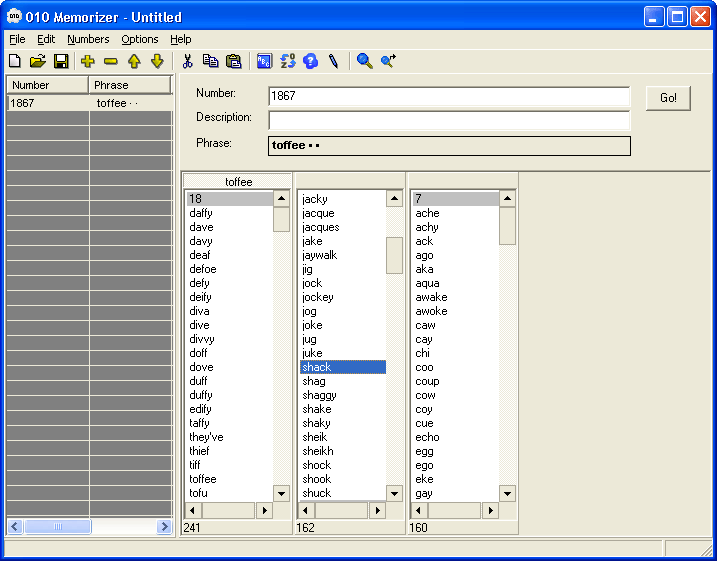
\includegraphics[draft=false,width=0.5\linewidth]{010Memorizer1}
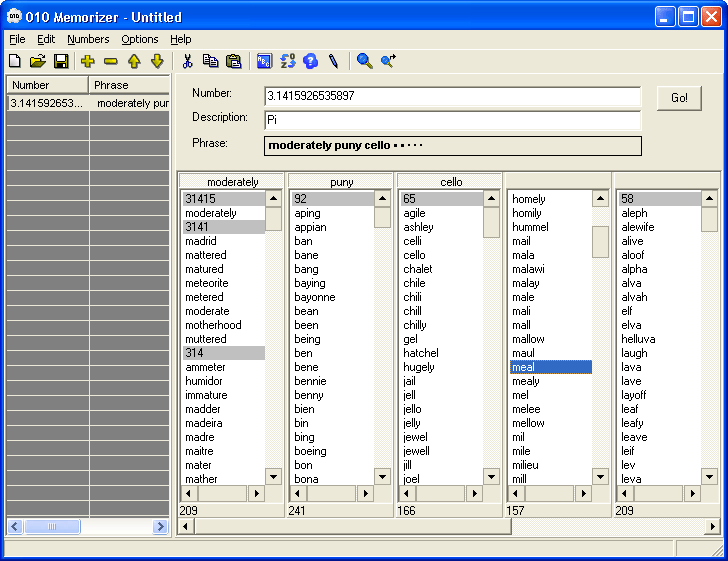
\includegraphics[draft=false,width=0.51\linewidth]{010Memorizer2}
\caption{Скриншот компьютерной программы 010Memorizer.}
\label{ris:image}
\end{figure}
\end{center}
\textbf{2Know} \cite{litlink7} — ещё одно приложение для Windows. Оно более простое в понимании и настройке, чем 010 Memorizer, однако в нём поддерживается меньшее число функций. Приложение позволяет ввести короткое число, которое необходимо запомнить, и получить список слов, соответствующих ему по основной мнемонической системе. Плюсы 2Know: простота использования, возможность выбрать среди несколько европейских языков. Минусы: устаревший дизайн, отсутствие возможности сохранить запоминаемые фразы, малое число функций.\\
\begin{figure}[h]
\center{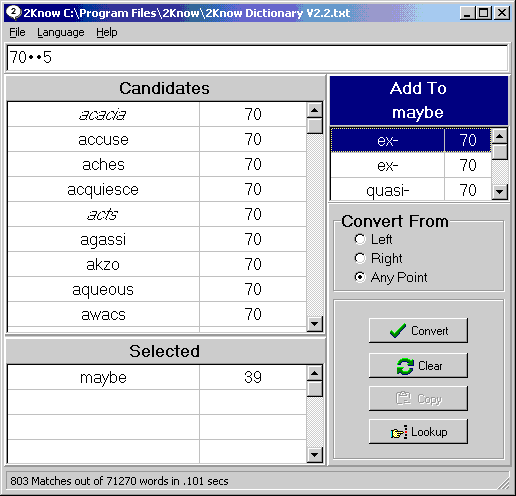
\includegraphics[draft=false,width=0.5\linewidth]{2Know}}
\caption{Скриншот приложения для компьютера 2Know.}
\label{ris:image}
\end{figure}\\
~\\
~\\
~\\
~\\
~\\
~\\
~\\
~\\
Самым популярным сайтом для Доминиканской мнемонической системы является \textbf{peoplebyinitials} \cite{litlink8}. Он позволяет вывести список людей, соответствующих нужным пользователю инициалам. При клике на каждого человека можно перейти на его страничку в Википедии. Рядом с каждым персонажем есть возможность указать его действия, чтобы легче запомнить. Сильными сторонами сайта являются минималистичный дизайн, проработанный удобный функционал, возможность настраивать собственные ассоциации. Слабые стороны peoplebyinitials: нет возможности сохранить выбранные ассоциации на сайте, их возможно только выгрузить в формате csv. Также невозможно выбрать другой язык, кроме английского.\\
\begin{figure}[h]
\center{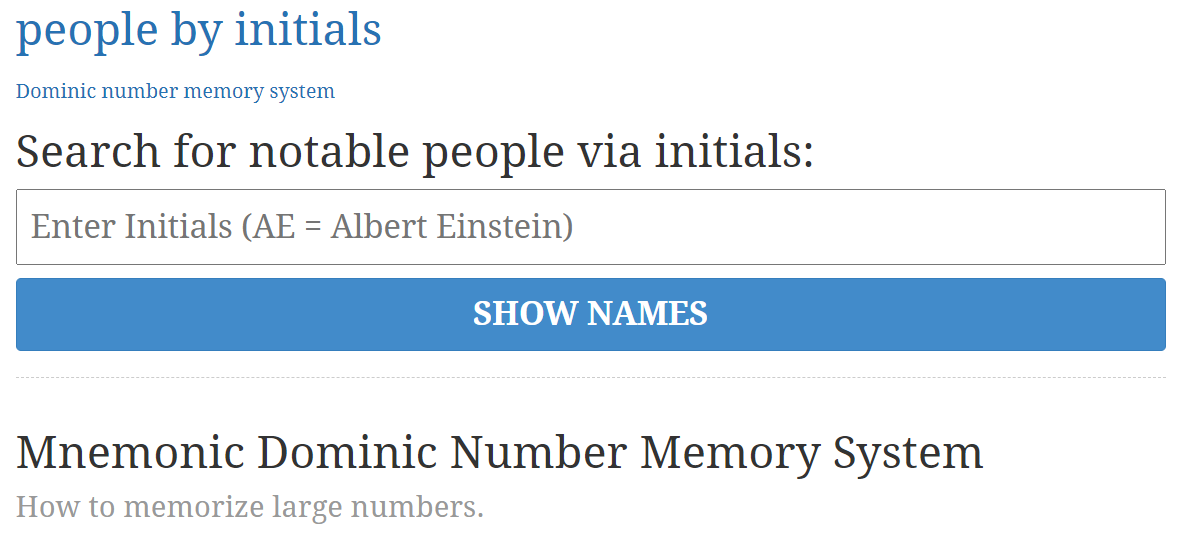
\includegraphics[draft=false,width=0.5\linewidth]{peoplebyinitials}}
\caption{Поиск имен в сервисе peoplebyinititals.}
\label{ris:image}
\end{figure}\\
\begin{figure}[h]
\center{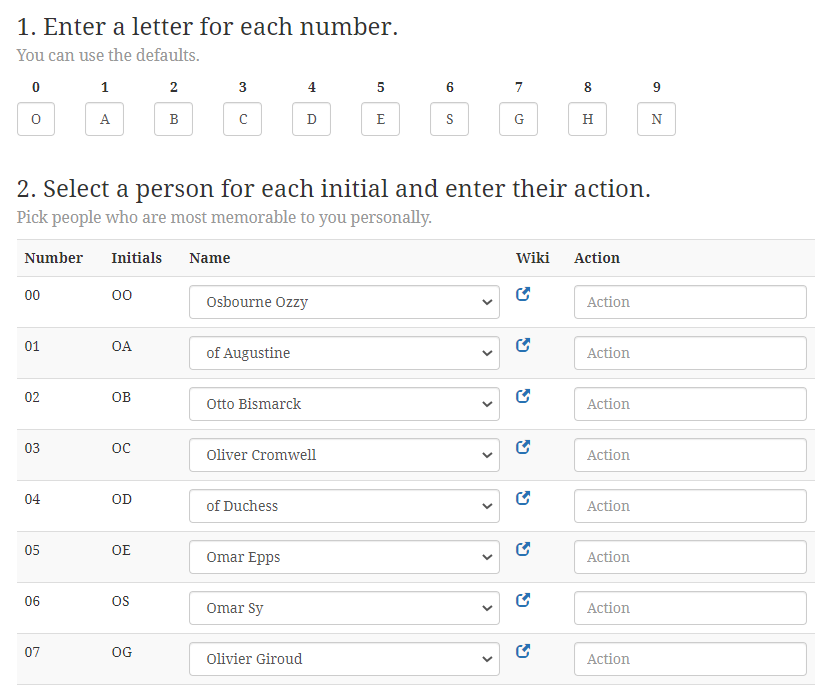
\includegraphics[draft=false,width=0.5\linewidth]{peoplebyinitials1}}
\caption{Пример работы сайта peoplebyinititals.}
\label{ris:image}
\end{figure}\\
~\\
~\\
~\\
~\\
~\\
~\\
~\\
~\\
~\\
~\\
~\\
Перейдём теперь к мобильным приложениям для мнемонических систем. По состоянию на декабрь 2022, около 5000 пользователей пользуются приложением \textbf{Mnemonic major system} \cite{litlink9}. В нём есть множество функций для использования основной мнемонической системы: запоминание ассоциаций для цифр, список составленных ассоциаций, различные квизы для быстрого запоминания. Плюсы приложения: разнообразие функций, гибкие настройки, удобный интерфейс. Минусы: устаревший дизайн, отсутствие поддержки других языков, кроме английского.\\
\begin{center}
\begin{figure}[h]
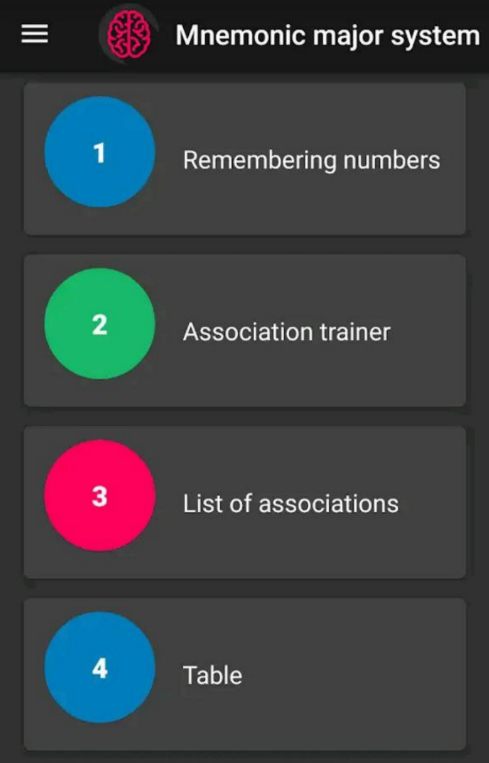
\includegraphics[draft=false,width=0.25\linewidth]{MnemonicMajorSystem1}
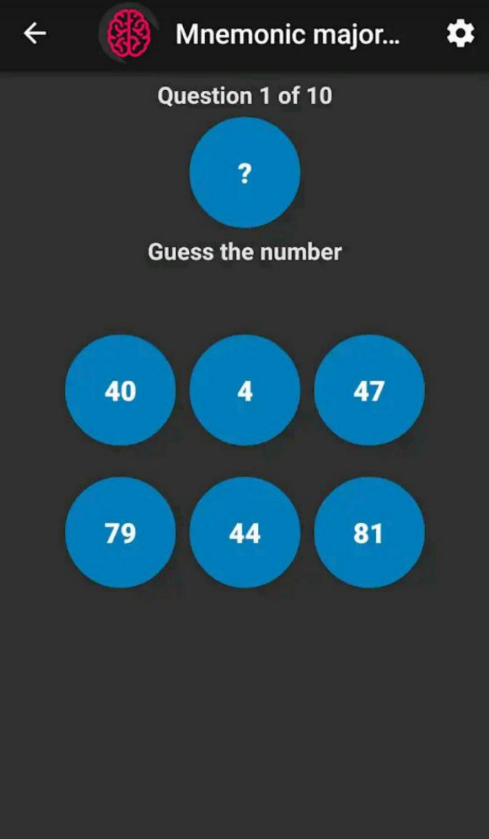
\includegraphics[draft=false,width=0.228\linewidth]{MnemonicMajorSystem2}
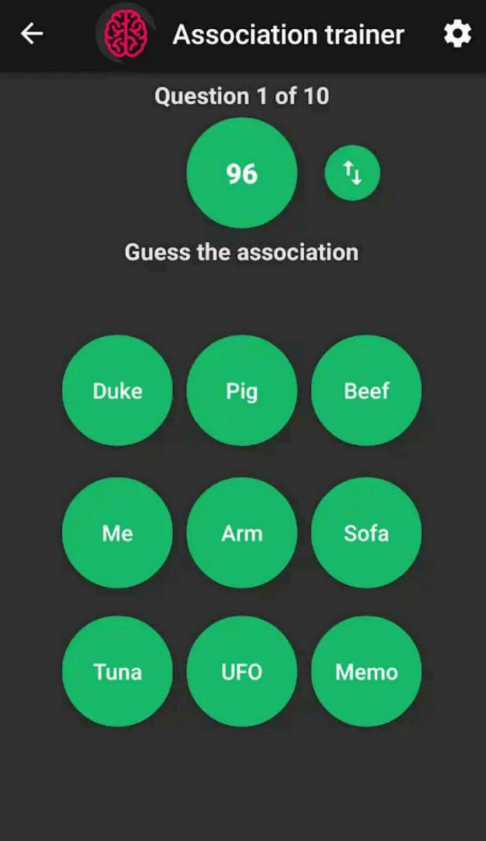
\includegraphics[draft=false,width=0.226\linewidth]{MnemonicMajorSystem3}
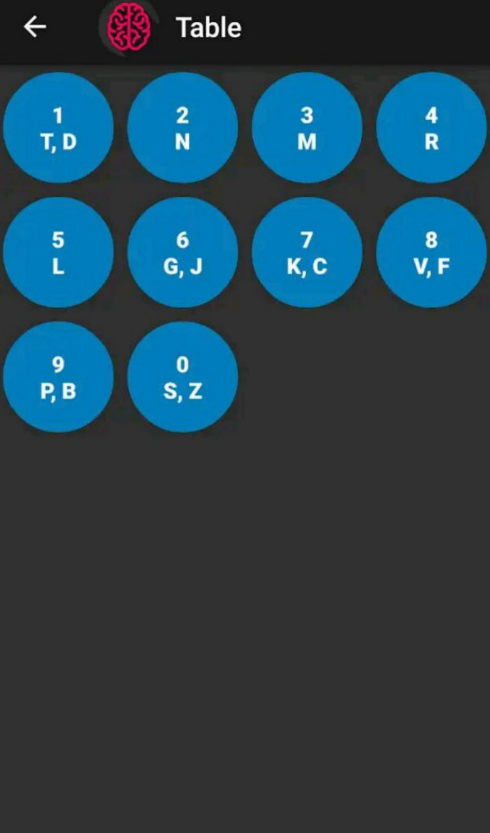
\includegraphics[draft=false,width=0.23\linewidth]{MnemonicMajorSystem4}
\caption{Скриншоты приложения Mnemonic major system.}
\label{ris:image}
\end{figure}
\end{center}
~\\
~\\
~\\
~\\
Мобильное приложение \textbf{«Major System: Word Generator»} \cite{litlink10} напоминает 010 Memorizer по своему функционалу. В нём можно ввести короткое число, которое необходимо запомнить и получить список слов, подходящих ему по основной мнемонической системе. Преимущества приложения: минималистичный дизайн, удобный список слов, возможность выбора из двух языков: английского и испанского.\\
\begin{figure}[h]
\begin{center}
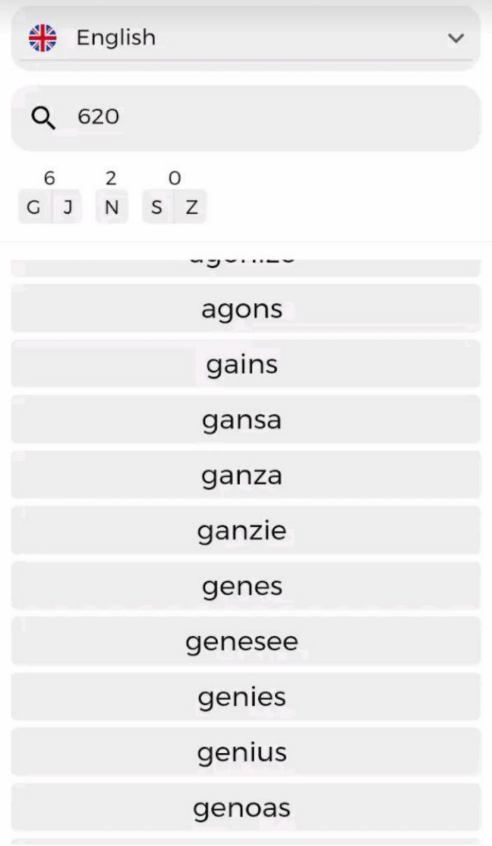
\includegraphics[draft=false,width=0.25\linewidth]{wordgenerator1}
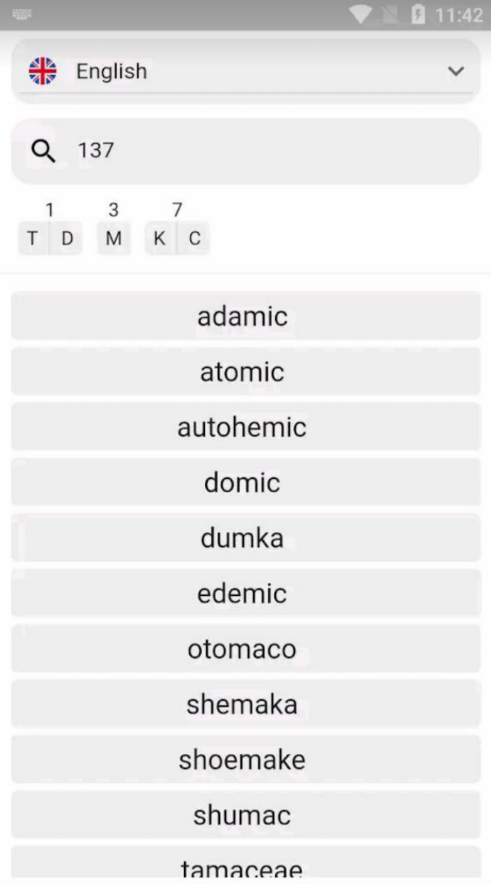
\includegraphics[draft=false,width=0.239\linewidth]{wordgenerator2}
\caption{Примеры работы приложения Major System: Word Generator.}
\label{ris:image}
\end{center}
\end{figure}
~\\
\textbf{A+ Major System} \cite{litlink11} — эргономичное приложение для удобного использования основной мнемонической системы. В нём есть возможность добавлять картинки к введённым словам, записывать числа, которые требуется запомнить. Важным преимуществом приложения является современный дизайн. Минус — малое количество поддерживаемых функций.\\
\begin{figure}[h]
\begin{center}
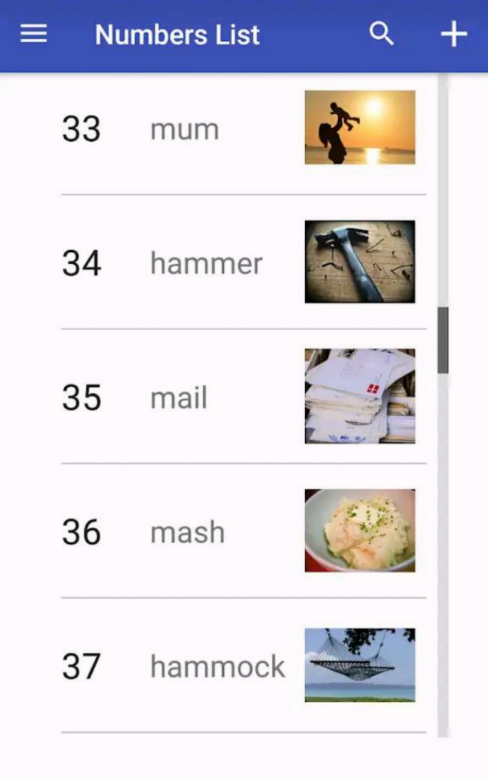
\includegraphics[draft=false,width=0.249\linewidth]{aplus1}
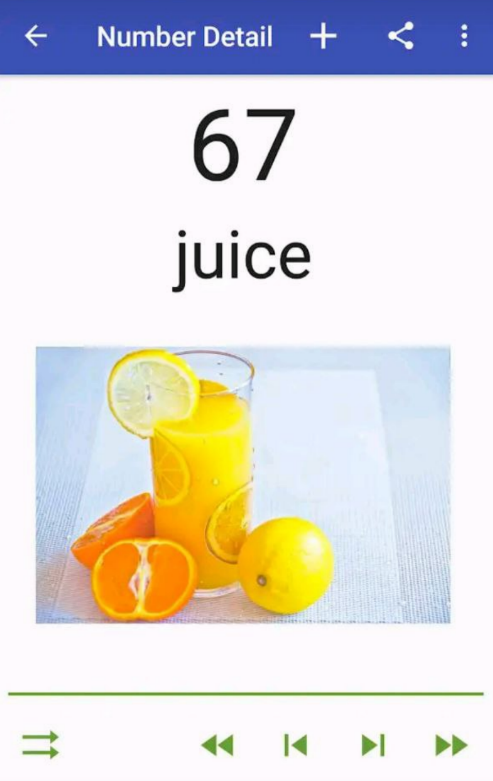
\includegraphics[draft=false,width=0.25\linewidth]{aplus2}
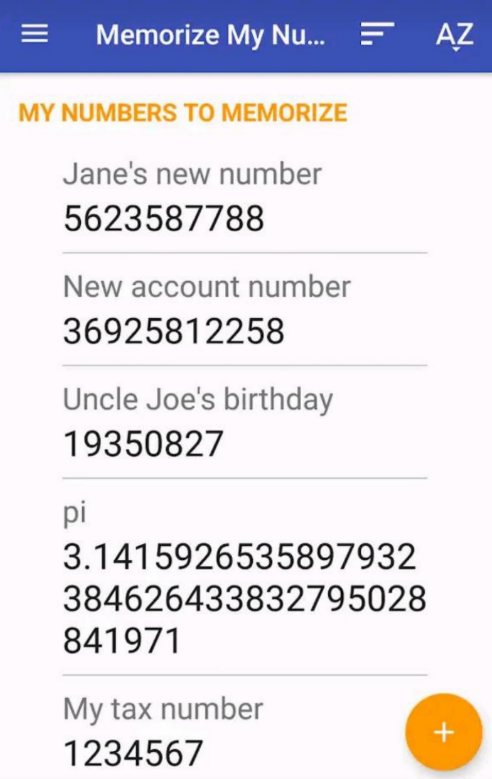
\includegraphics[draft=false,width=0.25\linewidth]{aplus3}
\caption{Скриншоты приложения A+ Major System.}
\label{ris:image}
\end{center}
\end{figure}
~\\
\textbf{Вывод из анализа конкурентов:}\\
Несмотря на то, что Доминиканская система показывает лучшие результаты, количество компьютерных сервисов, упрощающих работу с ней, значительно меньше, чем с основной мнемонической системой. Сервисы, позволяющие использовать и ту, и другую мнемонические системы, отсутствуют на рынке. Исследование конкурентов показывает, что в англоговорящей среде более распространена основная мнемоническая система, но в существующих приложениях для ее использования есть недостатки:
\begin{itemize}
\item Устаревший дизайн;
\item Небольшой выбор языков интерфейса;
\item Отсутствие возможности сохранения запоминаемых чисел;
\item Недостаточное количество функций.
\end{itemize}
\begin{center}
\subsection{Вывод}
\end{center}
В ходе интервью с потенциальными пользователями, а также в ходе анализа конкурентов были сделаны следующие выводы. Во-первых, в приложении необходима возможность выбора языка. Во-вторых, нужно дать пользователям информацию об обеих мнемонических системах, так как не все пользователи знают о них (информация появляется при явном запросе пользователя). В третьих, требуется создать общий список чисел, запоминаемых пользователем для периодического повторения. При выборе основной мнемонической системы необходимо реализовать поиск слов-ассоциаций по выбранным цифрам (соответствующие слова хранятся в пополняемой пользователем базе). При выборе Доминиканской системы — поиск известных личностей по их инициалам (список личностей хранится в пополняемой пользователем базе).\\
\newpage
\section {Назначение разработки}
\textbf{Целевая аудитория продукта:}\\
Люди, которым требуется запоминать большие числа на постоянной основе. Также приложением могут пользоваться люди, которые хотят улучшить свою память. Достаточно распространенными примерами чисел для запоминания являются номера клиента банка, номера банковских карт, номера страховых свидетельств, дни рождения, экстренные номера телефонов, телефоны знакомых, важные в программировании числа, исторические даты, слова иностранных языков, имена и лица. В связи со спецификой предоставляемой в приложении информации, ограничение на возраст пользователя — от 6 лет.\\
~\\
\textbf{Актуальность проблемы:}\\
Проблема запоминания больших чисел — вечная проблема, так как память человека не менялась значительно на протяжении истории. Поэтому приложение, позволяющее быстро запоминать числовые данные может быть полезно до тех пор, пока будут существовать мобильные телефоны.\\
~\\
\textbf{Функциональное назначение:}\\
Программа представляет из себя удобное приложение для хранения и запоминания чисел, а также изучения основной мнемонической и Доминиканской систем. Приложение не ограничивает пользователя в количестве сохраненных им чисел, ограничивающим фактором является только память телефона.\\
Приложение делится на 5 основных разделов:
\begin{itemize}
\item Запоминаемые числа;\\
\item Информация об основной мнемонической системе;\\
\item Справка;\\
\item Информация о Доминиканской системе;\\
\item Личный кабинет.\\
\end{itemize}
Более подробное описание элементов программы представлено в следующем разделе.\\
~\\
\textbf{Эксплуатационное назначение:}\\
Приложение предназначено для пользователей мобильных устройств от 6 лет. Доступ в интернет не является необходимым для работы программы.
~\\

\newpage
\section {Требования к программе или программному изделию}
\textbf{Краткое описание приложения}\\
Приложение должно позволить русскоговорящим пользователям применять основную мнемоническую и доминиканскую системы для запоминания больших чисел. Для этого должна быть реализована возможность выбора языка, используемого приложением. Создана справка, позволяющая узнать всю нужную информацию об обеих системах. Помимо этого, необходимо использовать карточки для выучивания связи между цифрами и буквами в обеих системах. Кроме того, будет реализована работа со словарем: пользователь сможет открывать используемый в приложении словарь и добавлять туда новые слова.\\
~\\
\textbf{Структура мобильного приложения}\\
Приложение состоит из 11 экранов (результат предварительного проектирования по состоянию на конец января 2023 года):
\begin{itemize}
\item \textbf{Запоминаемые числа}\\
На данном экране представлен список запоминаемых чисел в виде "{}плиток"{}\ — выделяющихся на фоне основного приложения прямоугольных элементов. На каждой из них расположена картинка, выбранная пользователем, если она есть. Под картинкой — его название и само число. В случае, если число не помещается в пределах плитки, оно сокращается до первых нескольких символов. В правой нижней части экрана присутствует кнопка "{}Добавить"{}\ , переводящая пользователя на следующий экран.
\item \textbf{Добавление числа}\\
При добавлении числа открывается экран с двумя полями ввода — описанием числа и самим числом. Также присутствует возможность выбора изображения из памяти телефона. На этой же странице присутствует выбор мнемонической системы среди вариантов: основная мнемоническая, Доминиканская, без системы.
\item \textbf{Поиск слов для запоминания}\\
В верхней части экрана указано пояснение: "{}Выберете цифры для поиска слов:"{}. Под ним отражены цифры указанного пользователем числа в виде кнопок. При нажатии поочередно каждой из этих кнопок, под ними появляется список слов, соответствующих выбранным цифрам в указанной мнемонической системе. При нажатие любого из этих слов, они добавляются в поле ввода в нижней части экрана. Под этим полем ввода присутствует кнопка "{}Сохранить число"{}.
\item \textbf{Редактирование числа}\\
При нажатии на любое из чисел в экране "{}Запоминаемые числа"{}\ открывается экран редактирования числа. На нем есть возможность изменить описание, число, фразу для запоминания в соответствующих текстовых полях. Также возможно выбрать другое фото. В нижней части экрана — кнопка "{}Сохранить"{}.
\item \textbf{Карточки с числами в основной мнемонической системе}\\
Этот экран нужен для того, чтобы позволить пользователю выучить соответствие между цифрой и буквой в основной мнемонической системе. Для этого на главном экране расположена прямоугольная карточка с изображением случайной цифры. При нажатии на нее она переворачивается, показывая соответствующую букву. При ее листании открывается следующая карточка.
\item \textbf{Справка с информацией об обеих системах}\\
На данном экране представлена информация об основной мнемонической и Доминиканской системах в виде текста, изображений, а также таблиц.
\item \textbf{Карточки с числами в доминиканской системе}\\
Экран нужен для того, чтобы позволить пользователю выучить соответствие между цифрой и буквой в Доминиканской системе. Для этого на главном экране расположена прямоугольная карточка с изображением случайной цифры. При нажатии на нее она переворачивается, показывая соответствующую букву. При ее листании открывается следующая карточка.
\item \textbf{Панель настроек}\\
Панель настроек отображает список из всех главных экранов, отраженных в нижнем меню, с их описаниями. Также присутствует "{}Выбор языка"{}\ и "{}Словарь"{}. Справа от каждого из пунктов настроек приведен соответствующий ему логотип.
\item \textbf{Список слов в словаре}\\
В верхней части экрана расположен поиск слов, под ним — список всех слов словаря в алфавитном порядке. В правой нижней части экрана присутствует кнопка "{}Добавить"{}, позволяющая добавить слово в словарь.
\item \textbf{Добавление слова в словарь}\\
Всплывающее окно с единственным полем ввода "{}введите слово"{}\ и кнопкой "{}Добавить"{}.
\item \textbf{Выбор языка}\\
Всплывающее окно с выпадающим списков языков и кнопкой "{}Выбрать язык"{}. В данный момент предоставляется выбор из двух языков: английского и русского.
\end{itemize}
Примерный вид описанных экранов может быть увиден в прототипе интерфейса, созданном в приложении Figma. См. приложение №2.\\
~\\
\textbf{Шаблон страницы}\\
Экран всегда вертикальный, разворот запрещен.\\
~\\
\textbf{Шапка}\\
Шапка страницы меняется в зависимости от текущей страницы. На ней появляется название страницы, а также иконка поиска, если это необходимо на текущей странице.\\
Для всех внутренних страниц (не обозначенных в нижнем меню) должна быть кнопка
Вернуться.\\
~\\
\textbf{Подвал}\\
Основное меню располагается в нижней части экрана. Разделы обозначаются иконками:
\begin{itemize}
\item Раздел "{}Запоминаемые числа"{} отражён с помощью иконки "{}123"{}, символизирующей числа.
\item Раздел "{}Карточки с числами в основной мнемонической системе"{}\ отражён иконкой "{}MMS"{}, означающей сокращение от названия "{}mnemonic major system"{}.
\item Раздел "{}Справка с информацией"{}\ символизируется вопросительным знаком.
\item Раздел "{}Карточки с числами в Доминиканской системе"{}\ отражаются икокной "{}DS"{}. Это сокращение от "{}Dominic system"{}.
\item Раздел настроек отражается классической шестеренкой, символизирующей настройки.
\end{itemize}
~\\
\textbf{Требование к интерфейсу}\\
Интерфейс должен быть оформлен в соответствии с дизайн-системой Material Design.\\
~\\
\textbf{Разрешения}\\
В данном приложении у пользователя спрашивается только одно разрешение — доступ к файловой системе. Оно должно впервые запрашиваться у пользователя при попытке добавить фотографию к числу.\\
~\\
\textbf{Дальнейшая работа}\\
Область применения обеих изучаемых в работе мнемонических систем обширна, поэтому приложение имеет множество возможностей для расширения. Дополнительные функции могут быть реализованы автором в том случае, если в срок будет реализован основной функционал.\\
В краткосрочной перспективе могут быть добавлены:
\begin{itemize}
\item Статистика, позволяющая пользователю отслеживать свои результаты;
\item Возможность делиться сохраненными числами с другими пользователями;
\item Отслеживание статистики друзей для создания соревновательного эффекта;
\end{itemize}
В случае востребованности приложения пользователями, появится смысл выходить на новые рынки. Для этого потребуется добавление нового функционала, а также перевода интерфейса приложения на другие языки.\\
В долгосрочной перспективе могут быть добавлены: 
\begin{itemize}
\item Поддержка других языков, кроме русского и английского;
\item Другие мнемонические системы, например, система Катапаяди;
\item Способы тренировки памяти для её улучшения.
\end{itemize}
\newpage
\section {Требования к программной документации}
Программная документация подготовлена в соответствии с требованиями к программным проектам студентов образовательной программы "{}Программная инженерия"{}.\\
~\\
При составлении документации использовался международный стандарт для подготовки технического описания программы IEEE Std 1016-1998 «IEEE Recommended Practice for Software Design Descriptions» \cite{litlink12}, а также ГОСТ 19 Единая система программной документации (ЕСПД) \cite{litlink13}.
\newpage
\section {Технико-экономические показатели}
\textbf{Первоначальная оценка успеха проекта:}\\
Соответствие написанного приложения заявленным требованиям (функциональное тестирование).\\
~\\
\textbf{Последующая оценка:}\\
Оценка приложения принимающей комиссией на защите курсовой работы в институте (ДПИ ФКН НИУ ВШЭ).\\
~\\
\textbf{Конечный параметр оценки проекта:}\\
Число пользователей, установивших приложение в магазине приложений Google Play.\\
\newpage
\section {Стадии и этапы разработки}
\textbf{Ноябрь:}
\begin{itemize}
\item Анализ источников;
\item Анализ user stories;
\item Анализ аналогов;
\item Получение полной информации о требуемой функциональности.
\end{itemize}
\textbf{Декабрь:}
\begin{itemize}
\item Создание макета приложения в figma;
\item Создание технического задания;
\item Драфт пояснительной записки.
\end{itemize}
\textbf{Январь:}
\begin{itemize}
\item Начало работы над приложением;
\item Завершение пояснительной записки.
\end{itemize}
\textbf{Февраль:}
\begin{itemize}
\item Создание основного функционала приложения (разработка);
\item Контрольная точка 1 — представление ТЗ.
\end{itemize}
\textbf{Март:}
\begin{itemize}
\item Создание дополнительного функционала приложения;
\item Исправление ошибок;
\item Создание презентации, подготовка к выступлению перед комиссией.
\end{itemize}
\textbf{Апрель:}
\begin{itemize}
\item Окончательное оформление документов;
\item Загрузка документов;
\item Защита курсовой (ориентировочно 15-17 апреля).
\end{itemize}
\newpage
\section {Порядок контроля и приемки}
\textbf{Выбор темы курсовой:}\\
До 15 февраля можно выбрать тему и руководителя проекта или поменять тему/руководителя проекта.\\
~\\
\textbf{В случае опоздания с выбором темы или руководителя:}
\begin{enumerate}
\item Заполните форму Объяснительной записки;
\item Ждите открытия доступа к загрузке (придет сообщение на учебную почту);
\item Загружайте в блок "{}Заявление на выбор темы и руководителя проекта 2022/2023"{}\ заявление и описание проекта в формате .DOCX (Если проект не согласован для вашей ОП и курса в таблице, на заявлении обязательно должна быть подпись Шилова В. В.).
\end{enumerate}
\textbf{Этап 2. Контрольная точка 1}\\
К данному этапу выполнения проекта необходимо подготовить техническое задание (ТЗ).\\
~\\
\textbf{ВАЖНЫЕ ДАТЫ:}
\begin{itemize}
\item До 1 февраля 2023 - Отправить руководителю Отчет на проверку;
\item До 8 февраля 2023 - получить обратную связь от руководителя и приступить к исправлению недочетов;
\item До 15 февраля 2023 23:59 - загрузить документы в блок "{}Этап 2. Контрольная точка 1"{}\ в SmartLMS.
\end{itemize}
\newpage
\addcontentsline{toc}{section}{Список использованных источников}
\section*{Список использованных источников}
\begin{thebibliography}{}
\bibitem{litlink1} \textit{AndroidDev} (2022) Meet Android Studio // Сайт developer.android.com (https://developer.android.com/studio/intro) Просмотрено: 27.01.2023.
\bibitem{litlink2} \textit{AndroidDev} (2022) Get Android Studio // Сайт developer.android.com (https://developer.android.com/studio) Просмотрено: 27.01.2023.
\bibitem{litlink3} \textit{David Phair (PhD) and Alexandra Shaeffer (PhD)} (2022) The “Golden Thread” Explained Simply // Сайт gradcoach.com. Июнь (https://gradcoach.com/research-aims-objectives-questions/)
\bibitem{litlink4} \textit{Dr Adani Pujada, Dr Sunni Patel, Daisy Shearer} (2022) Aims and Objectives – A Guide for Academic Writing // Сайт discoverphds.com. (https://www.discoverphds.com/advice/doing/research-aims-and-objectives)
\bibitem{litlink5} \textit{Chaitanya Shinkhede, Priya Chetty} (2021) Difference between thesis objectives and research questions // Сайт projectguru.in. 8 ноября (https://www.projectguru.in/difference-between-thesis-objectives-and-research-questions/)
\bibitem{litlink6} \textit{SweetScape Software Inc.} (2022) 010 Memorizer - Memorize Numbers with Ease // Сайт sweetscape.com (https://www.sweetscape.com/010memorizer/) Просмотрено: 27.01.2023.
\bibitem{litlink7} \textit{Team Got2Know} (2013) Unforgettable Software // Сайт got2know.net. 16 марта (http://www.got2know.net/) Просмотрено: 27.01.2023.
\bibitem{litlink8} \textit{\_enzo\_dev} (2014) People By Initials // Сайт madebyenzo.com. 30 марта (https://madebyenzo.com/posts/people-by-initials/) Просмотрено: 27.01.2023.
\bibitem{litlink9} \textit{RavarApp} (2019) Mnemonic major system // Сайт play.google.com. 10 марта (https://play.google.com/store/apps/details?id=com.ravarapp.mnemonic\_major\_system) Просмотрено: 27.01.2023.			
\bibitem{litlink10} \textit{Zereck} (2021) Major System: Word Generator // Сайт play.google.com. 11 сентября (https://play.google.com/store/apps/details?id=com.zereck.major\_system\_word\_generator)
\bibitem{litlink11} \textit{Magic Parcel} (2018) A+ Major System // Сайт play.google.com. 19 мая (https://play.google.com/store/apps/details?id=com.magicparcel.app.majorsystem)
\bibitem{litlink12} \textit{IEEE} (1998) IEEE Recommended Practice for Software Design Descriptions // Сайт ieeexplore.ieee.org. 4 декабря (https://ieeexplore.ieee.org/document/741934)
\bibitem{litlink13} ГОСТ 19.001-77. Единая система программной документации. Термины и определения: утвержден и введен в действие Постановлением Государственного комитета стандартов Совета Министров СССР от 20 мая 1977 г. № 1268 срок введения: с 01.01.1980 г. – URL: https://www.swrit.ru/doc/espd/19.001-77.pdf (дата обращения: 27.01.2023). – Текст: электронный.
\end{thebibliography}
\newpage
\begin{center}
\addcontentsline{toc}{section}{Приложения}
\section*{Приложения}
\end{center}
\zz{}\textbf{Приложение 1\\}
Ссылка на репозиторий проекта с исходным кодом и всеми использованными материалами.\\
https://github.com/NikPeg/mnemonic\_systems\_app\\
\zz{}\textbf{Приложение 2\\}
Ссылка на проект интерфейса в сервисе Figma, отражающий примерную структуру будущего приложения.\\
https://www.figma.com/file/jBcJmt0PREwHvBQRowhaHO/Mnemonic-systems?node-id=38\%3A250\&t=\\
Q8JXDdb3HXM9gGPh-1\\
\end{document}